% \chapter{Technical Fundamentals}
% Since the main part of this thesis addresses the implementation of flow control algorithms for a left ventricular assist device, the basics of control theory and a introduction on iterative learning control will be presented here as well.

\chapter{Control Theory}
Since this thesis addresses the implementation of flow control algorithms for a left ventricular assist device, this section will focus on the fundamentals of notation and structure of a standard control loop. Furthermore, the basic principles of PI-controllers and  iterative learning control (ILC) are discussed, since these are used within the practical part of the thesis.
\section{Fundamentals}
The basic task of control engineering is to externally influence a time-varying process with the goal of executing the process in a predetermined manner. A control system is characterized in particular by the feedback of the controlled variable to the reference variable. The reference variable comprises the state that has to be achieved.
In theory, this is represented by a control loop with the components shown in \figurename~{\ref{fig:control_loop}}.
\begin{figure}
  \centering
  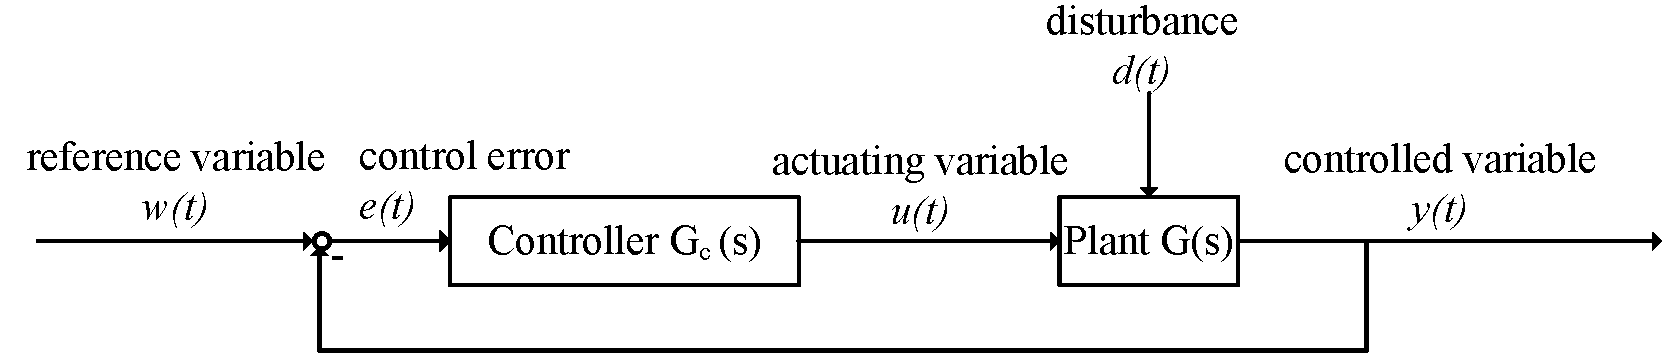
\includegraphics[width=0.9\textwidth]{images/chapt_3/control_loop.pdf}
  \caption[General structure of a control loop]{General structure of a control loop}
  \label{fig:control_loop}
\end{figure}
The plant $G(s)$ transfers the actuating variable $u(t)$, as well as the influence of the the disturbance $d(t)$, to the controlled variable $y(t)$. This variable is permanently compared with the reference variable $w(t)$ by means of a feedback loop, providing the control error
\begin{equation}
  e(t) = w(t) - y(t).
 \label{eq:e_t}
\end{equation}
The controller $G_{\mathrm{c}}(s)$ then transforms the control error to the actuating variable again. The aim of the control loop is to achieve the smallest possible control error with the highest possible damping. Since these goals contradict each other, a trade off must always be accepted here. \cite{Reg_17}
\\However, there are some general requirements for the closed control loop which have to be fulfilled. The first requirement states that the closed loop needs to be stable, which is met if the control loop responds to a finite excitation with a finite output signal. The second condition is the requirement for disturbance rejection, stating that the controlled variable needs to follow the reference variable asymptotically, so that
\begin{equation}
    \lim\limits_{t \rightarrow \infty}{e(t)} = 0.
 \label{eq:lim_e}
\end{equation}
Another requirement is that the dynamic relationship between the reference variable $w(t)$ and the controlled variable $y(t)$ must satisfy specified quality requirements.  Finally, these three requirements must be satisfied despite uncertainties in the plant, forming the robustness requirement. More detailed information on these requirements can be found in \cite{Reg_10}.

The plant $G(s)$ corresponds to the part of the system in which the physical quantity to be controlled is influenced by the controller. The calculation of the plant by setting up and solving differential equations is possible only in a few cases. Furthermore, calculation in many cases is very time consuming. Due to this, the determination of the plant's characteristic values is usually carried out experimentally. There are several basic types of plants, classified according to their dynamic behavior. As only the PT$_{\mathrm{1}}$-element is used in the practical part of this thesis, all other variations will not be discussed at this point. Detailed information on this topic can be found in \cite{Reg_10}.
\\The PT$_{\mathrm{1}}$-element is the plant type which is most common in technical equipment. A PT$_{\mathrm{n}}$-element in its steady state reacts proportionally to the input value and has a distinct transition behavior. The index n describes the order of the system. Therefore, a PT$_{\mathrm{1}}$-element is a proportional delay element of first order. The mathematical formulation of the transfer function of a PT$_{\mathrm{1}}$-element is
\begin{equation}
    G(s) = \frac{k_{\mathrm{s}}}{1+sT}.
 \label{eq:tf_pt1}
\end{equation}
The value $k_{\mathrm{s}}$ describes the static gain, which for a unit step and $h(t=0)=0$ is defined as
\begin{equation}
  k_{\mathrm{s}} = h(t\rightarrow \infty).
\end{equation}
 The time constant T gives an impression of the speed with which the system can react to changes at the input. It is defined as the time at which the transfer function reaches $63\, \%$ of its static gain. \cite{Reg_10}
\figurename~\ref{fig:tf_pt1} shows the transfer function of a PT$_{\mathrm{1}}$-element (blue curve) and its significant parameters.
\begin{figure}[ht]
   \centering
   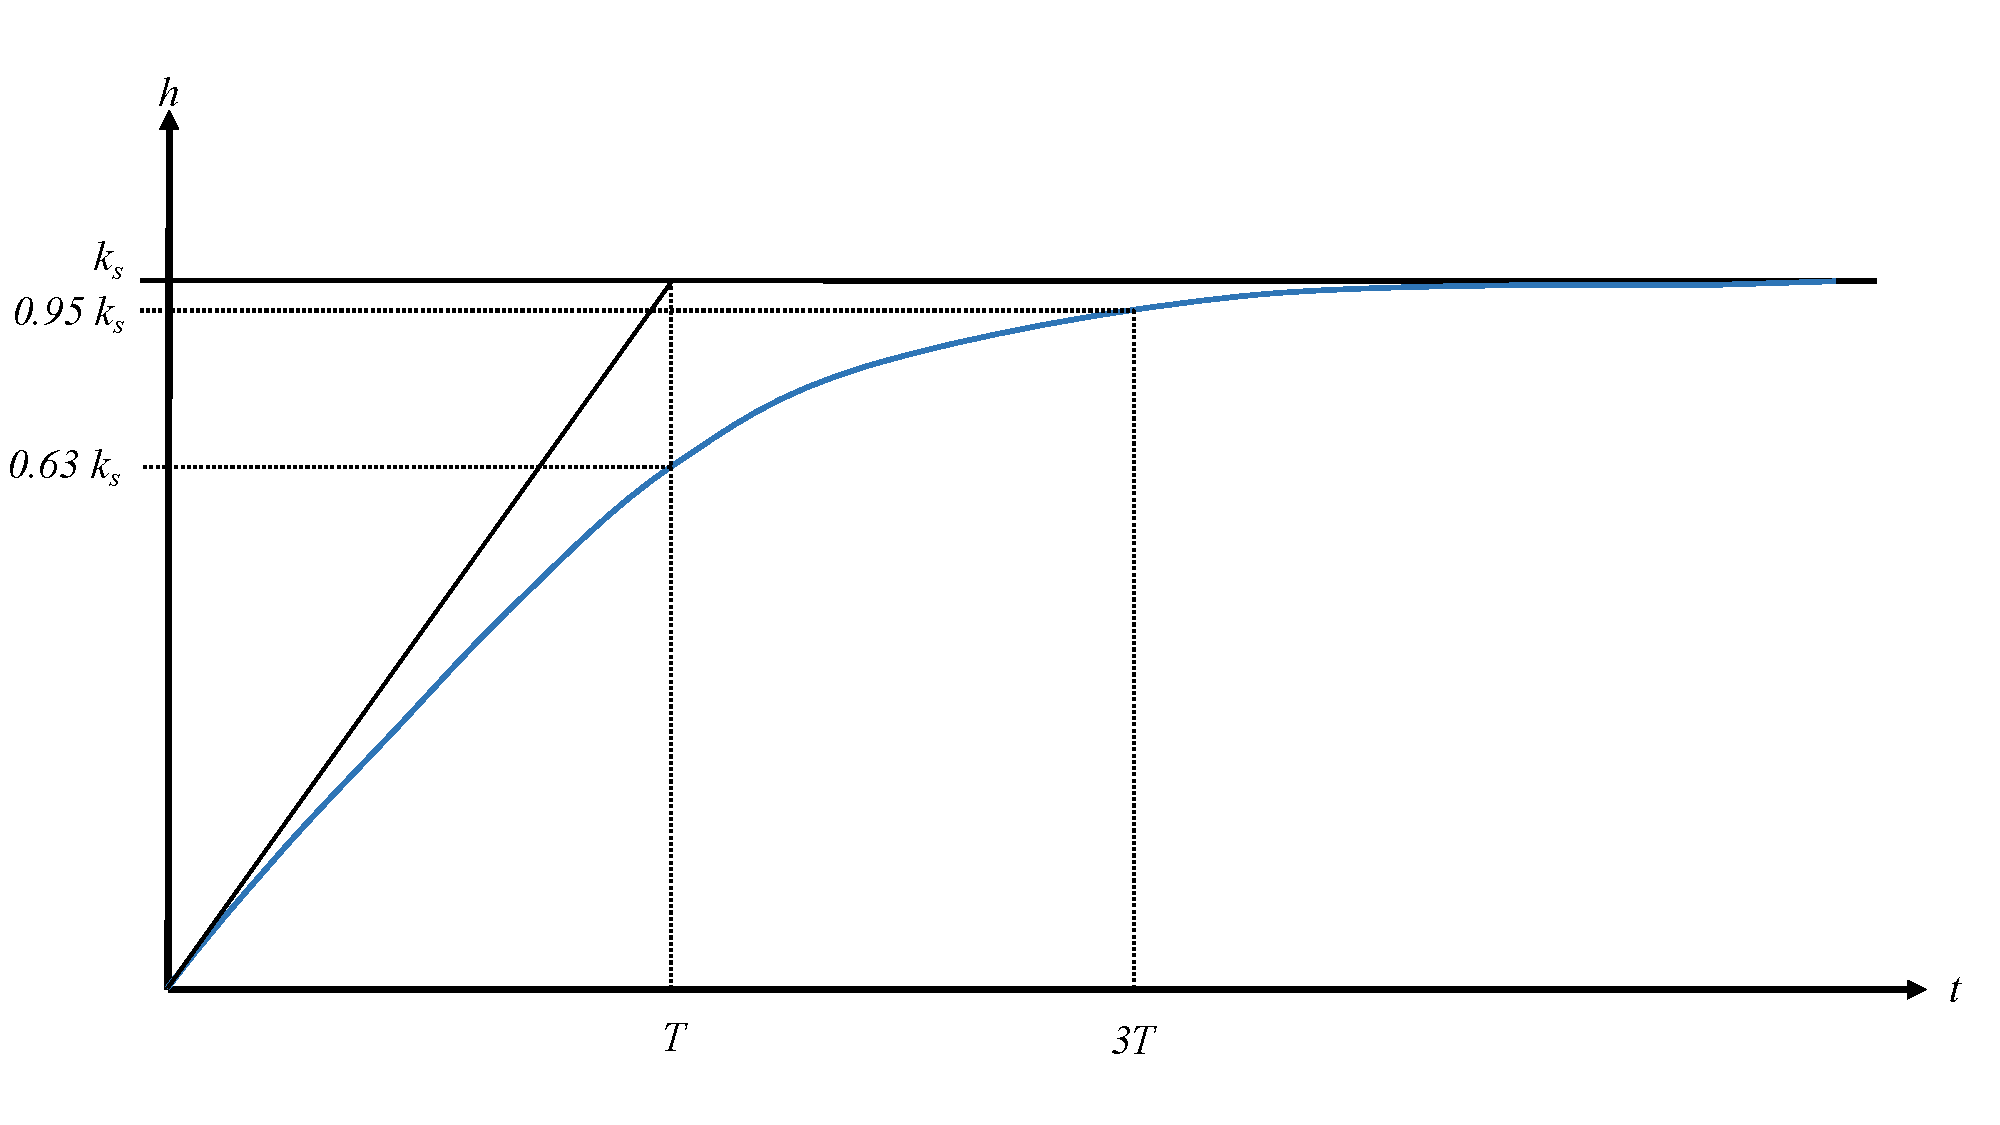
\includegraphics[width=\textwidth]{images/chapt_3/tf_pt1.pdf}
   \caption[Transfer function of a PT$_{\mathrm{1}}$-element]{Transfer function of a PT$_{\mathrm{1}}$-element \cite{Reg_10}.}
   \label{fig:tf_pt1}
 \end{figure}

\section{PI-controller}
A PI-controller is a control structure commonly used for linear systems. This structure consists of both a proportional (P) and an integral (I) control element.
The output value of a P-controller is proportional to its input value. In relation to the control loop in \figurename~\ref{fig:control_loop} this leads to
\begin{equation}
    u(t) = K_{\mathrm{P}}e(t).
 \label{eq:p_contr_1}
\end{equation}
\newpage
Using Laplace transformation, the transfer function for a P-controller can be determined as
\begin{equation}
    G(s) = \frac{u(s)}{e(s)} = K_{\mathrm{P}}.
 \label{eq:p_contr_2}
\end{equation}
Therefore, the step response of this controller equals a step weighted with the parameter $K_{\mathrm{P}}$.
\\The relationship between input and output value of an I-controller is described through
\begin{equation}
    u(t) = K_{\mathrm{I}}\cdot\int e(t) dt.
 \label{eq:i_contr_1}
\end{equation}
Just as for the P-controller, Laplace transformation can be used to determine the transfer function of the I-controller.
This leads to
\begin{equation}
    G(s) = \frac{u(s)}{e(s)} = \frac{K_{\mathrm{I}}}{s},
 \label{eq:i_contr_2}
\end{equation}
which indicates a step response in form of a ramp with slope $K_{\mathrm{I}}$.
In order to generate a PI-controller, the elements from (\ref{eq:p_contr_1}) and (\ref{eq:i_contr_1}) can be added, which leads to
\begin{equation}
    u(t) = K_{\mathrm{P}}e(t) + K_{\mathrm{I}}\cdot\int e(t) dt.
 \label{eq:pi_contr_1}
\end{equation}
Laplace transformation can be used again to compute the transfer function
\begin{equation}
    G(s) = \frac{u(s)}{e(s)} =  K_{\mathrm{P}} + \frac{K_{\mathrm{I}}}{s}.
 \label{eq:pi_contr_2}
\end{equation}
The step response of the PI-controller, illustrated in \figurename~\ref{fig:step_resp_pi}, shows both the weighted step from the P-controller and the ramp from the I-controller.

\begin{figure}[ht]
   \centering
   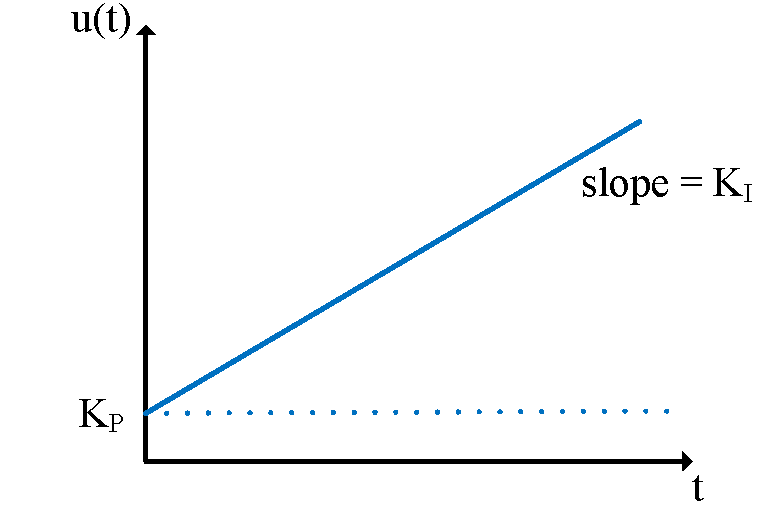
\includegraphics[width=0.6\textwidth]{images/chapt_3/step_resp_pi.pdf}
   \caption[Step response of a PI-Controller]{Step response of a PI-Controller based on \cite{Reg_17}.}
   \label{fig:step_resp_pi}
 \end{figure}

\subsection{Tuning rules}
Tuning the controller parameters, i.e adjusting their values depending on the system, is of great importance. Incorrectly chosen parameters can lead to poor performance or unstable system behavior, which may result in system damage. There are many different approaches to tune a PI-Controller in order to achieve optimal system performance. These range from heuristic methods over analysis of pole-zero plots to computer-aided numerical parameter optimization. \cite{Reg_10} At this point, the tuning rules according to Ziegler Nichols (ZN) and the rules according to Chien Hrones Reswick (CHR) will be discussed, as these are used for the implementation of flow control in the practical work. Information on other approaches can be found in \cite{Reg_11}.

\subsubsection{Tuning rules according to Ziegler Nichols} \label{chap:ZN}
The tuning rules according to Ziegler Nichols are one of the most commonly used heuristic methods in tuning controller parameters for PI-controllers. They are used especially if a mathematical model of the plant is not available but the plant can be approximated as a PT$_{\mathrm{n}}$-element. \cite{Reg_17}
A necessary condition is the possibility to experimentally identify the step response of the plant without risk of damage to the system. After the step response has been determined, it is displayed graphically. Then the inflection tangent is drawn into the step response as shown in \figurename~\ref{fig:param_zn}. The blue line represents the step response, the red line the inflection tangent, respectively.
\begin{figure}
   \centering
   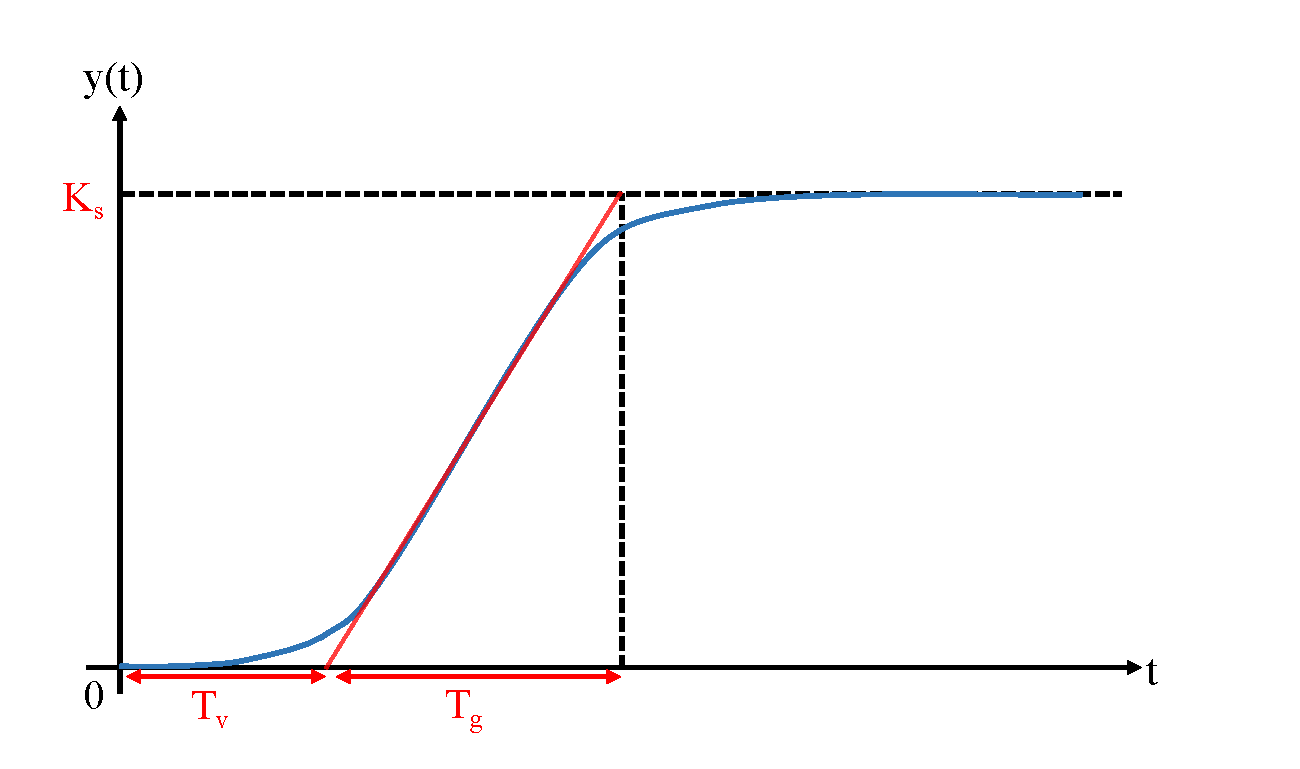
\includegraphics[width=0.8\textwidth]{images/chapt_3/param_zn.pdf}
   \caption[Inflection tangent method for Ziegler Nichols and Chien Hrones Reswick]{Inflection tangent method for Ziegler Nichols and Chien Hrones Reswick based on \cite{Reg_17}.}
   \label{fig:param_zn}
 \end{figure}
The gain $K_{\mathrm{S}}$, the delay time $T_{\mathrm{v}}$ and the settling time $T_{\mathrm{g}}$ can be read from the graph.
% The calculation of the controller parameters is performed according to the data in \tablename~\ref{tab:param_zn}.
Using these, following \cite{Reg_17}, the factor $K_{\mathrm{P}}$ is calculated as
\begin{equation}
  K_{\mathrm{P}} = 0.9\cdot\frac{T_{\mathrm{g}}}{K_{\mathrm{S}}T_{\mathrm{v}}}.
  \label{eq:kp_zn}
\end{equation}
The factor $K_{\mathrm{I}}$ is calculated according to:
\begin{equation}
    K_{\mathrm{I}}  = \frac{K_{\mathrm{P}}}{T_{\mathrm{N}}},
 \label{eq:K_I}
\end{equation}
with
\begin{equation}
    T_{\mathrm{N}}  = 3.3\cdot T_{\mathrm{v}}.
 \label{eq:T_N_zn}
\end{equation}
% \begin{table}
%   \centering
%   \begin{tabularx}{0.6\textwidth}{c|c|c|c}
%     \toprule
%     Controller type & $K_{P}$ &  $T_{N}$ & $T_{D}$   \\
%     \midrule
%     % P-Controller &  $\frac{T_{g}}{K_{S}T_{v}}$ & - & - \\
%     % & & & \\
%     PI-Controller & $0.9\frac{T_{g}}{K_{S}T_{v}}$ & $3.33T_{v}$ & - \\
%     % & & & \\
%     % PID-Controller & $0.9\frac{T_{g}}{K_{S}T_{v}}$ & $2T_{v}$ & $0.5T_{v}$ \\
%      \bottomrule
%   \end{tabularx}
%   \caption[Tuning parameters Ziegler Nichols]{Tuning parameters according to Ziegler Nichols}
%   \label{tab:param_zn}
% \end{table}

\subsubsection{Tuning rules according to Chien Hrones Reswick}\label{chap:CHR}
The tuning method according to Chien Hrones Reswick is very similar to the one by Ziegler Nichols. However, this method provides the ability to adjust the transient response of the control loop. The tuning parameters can either be chosen in a way to provide an overdamped behavior or a course providing $20\, \%$ overshoot. \cite{Reg_11}
For both options, the step response and its inflection tangent are graphically displayed, as for the Ziegler Nichols approach in \figurename~\ref{fig:param_zn}.
The values for $K_{\mathrm{S}}$, $T_{\mathrm{v}}$ and $T_{\mathrm{g}}$ can be read from the plot. The parameter value $K_{\mathrm{I}}$ again is calculated following (\ref{eq:K_I}). The formulas for calculating  $K_{\mathrm{P}}$,  $T_{\mathrm{N}}$ and $T_{\mathrm{D}}$ are given in \tablename~\ref{tab:param_chr}.

\begin{table}[ht]
  \centering
  \begin{tabular}{cc|cc}
    \toprule
     \multicolumn{2}{c|}{overdamped} & \multicolumn{2}{c}{20\% overshoot} \\
    \midrule
    $K_{\mathrm{P}}$ &  $T_{\mathrm{N}}$ & $K_{\mathrm{P}}$ &  $T_{\mathrm{N}}$ \\
    \midrule
     $0.35 \cdot \frac{T_{\mathrm{g}}}{K_{\mathrm{S}}T_{\mathrm{v}}}$ & $1.2 \cdot T_{\mathrm{v}}$  & $0.6 \cdot \frac{T_{\mathrm{g}}}{K_{\mathrm{S}}T_{\mathrm{v}}}$ & $T_{\mathrm{v}}$ \\
    \bottomrule
\end{tabular}
  \caption[Tuning parameters according to Chien Hrones Reswick]{Tuning parameters according to Chien Hrones Reswick based on \cite{Reg_17}.}
  \label{tab:param_chr}
\end{table}

\section{Iterative Learning Control}\label{ILC}
The use of iterative learning control aims to improve control performance for systems which execute the same task repeatedly under constant operating conditions. This improvement is based on the idea that it is possible to include error information from previous iterations into the adjustment of the actuation variable during the current iteration.
The standard control structure of an ILC algorithm is presented in \figurename~\ref{fig:ILC_only}.
\begin{figure}[ht]
   \centering
   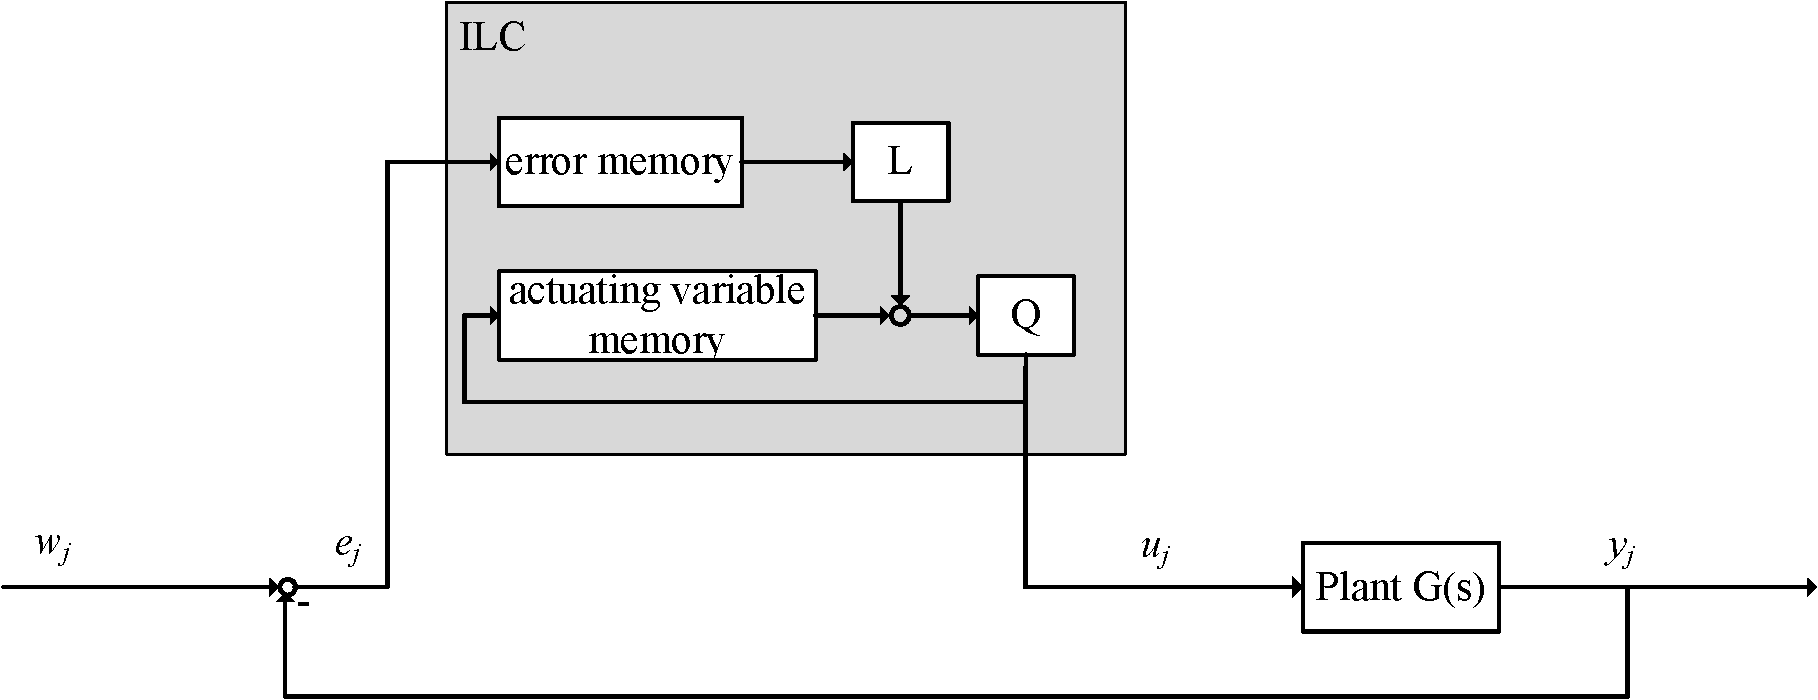
\includegraphics[width=0.9\textwidth]{images/chapt_3/ILC_only.pdf}
   \caption[Standard ILC control loop]{Standard ILC control loop based on \cite{ILC2}.}
   \label{fig:ILC_only}
 \end{figure}
\\Considering a linear-time-invariant single-input-single-output (SISO) system, the ILC learning algorithm is as follows:
\begin{equation}
    u_{\mathrm{j+1}}  = Q(q)[u_{\mathrm{j}}(k)+L(q)e_{\mathrm{j}}(k+1)]
 \label{eq:ILC_standard}
\end{equation}
where $k$ is the time index, $j$ is the iteration index, $q$ is the forward time-shift operator $qx(k) \equiv x(k + 1)$, $Q(q)$ is defined as the Q-Filter and $L(q)$ represents the learning function. The performance error signal $e_{\mathrm{j}}$ is defined as
\begin{equation}
    e_{\mathrm{j}}  = w_{\mathrm{j}}-y_{\mathrm{j}}.
 \label{eq:perf_error}
\end{equation}

 Feedback controllers such as PI-controllers are only able to consider the current changes in control error. By taking into account the information from previous iterations, low tracking errors are achievable through an ILC. This results in exceptional performance with convergence during the first few iterations. This can be achieved even for systems prone to repeating disturbances and model uncertainties. While feedback control shows a lag in transient tracking due to reacting to inputs and disturbances, ILC, as a feedforward controller, does not. Another advantage of ILC use is that there is no need for disturbances to be known or measured, as long as these signals show repeating behavior during each iteration. Furthermore, by storing signal information during each iteration, ILC enables advanced filtering and signal processing of the control error. However, ILC utilization holds some issues in regard to non-repeating disturbances or noise influences. In these cases it may be useful to combine ILC approaches with a feeback controller. A combination of the systems is furthermore required if the behavior of the plant is not stable. \cite{ILC2} A parallel architecture of a feedback controller in combination with an ILC is illustrated in \figurename~\ref{fig:ILC_parallel}.
 \begin{figure}[ht]
    \centering
    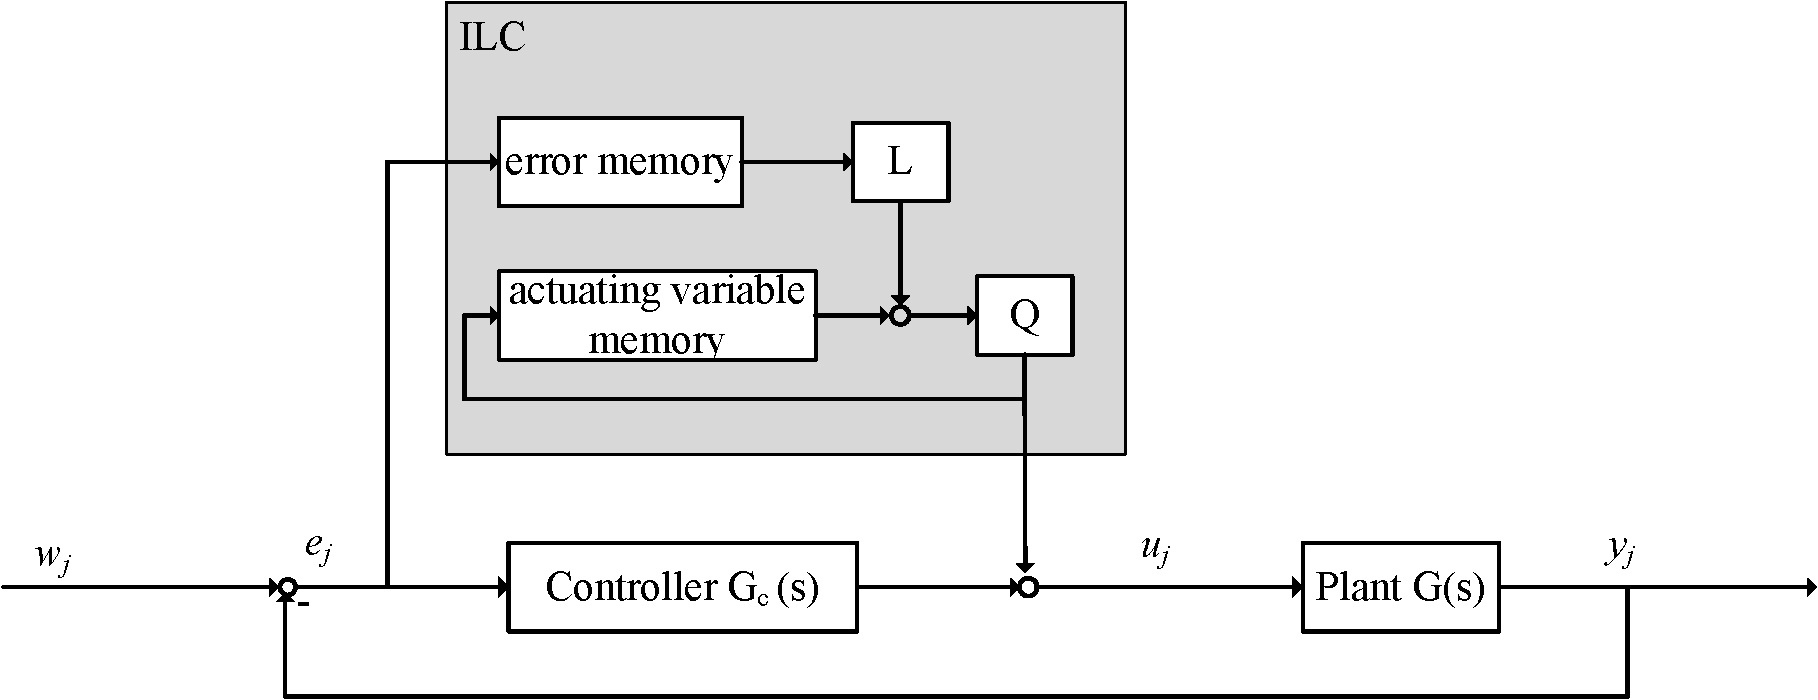
\includegraphics[width=0.9\textwidth]{images/chapt_3/ILC_parallel.pdf}
    \caption[Parallel architecture of ILC with feedback controller]{Parallel architecture of ILC with feedback controller based on \cite{ILC2}.}
    \label{fig:ILC_parallel}
  \end{figure}
\\There are several approaches to design an ILC. In general, an ILC ideally learns only the repeating disturbance patterns without being influenced by noise. The most common types of ILC learning functions are the P-, D- and PD-type learning functions. As an ILC does have a natural integrator action from one iteration to the next, I-type learning functions are rarely used.
\\The discrete-time learning function for a standard PD-type ILC is given as
 \begin{equation}
     u_{\mathrm{j+1}}(k) = u_{\mathrm{j}}(k)+k_{\mathrm{p}}e_{\mathrm{j}}(k)+k_{\mathrm{d}}[e_{\mathrm{j}}(k+1)-e_{\mathrm{j}}(k)].
  \label{eq:PD_type_2}
  \end{equation}
$k_{\mathrm{p}}$ represents the proportional gain while $k_{\mathrm{d}}$ is the derivative gain. In case a P-type learning function is implemented, the derivation gain is set to $k_{\mathrm{d}}=0$. For a D-type learning function, $k_{\mathrm{p}}=0$ is used, respectively.
\\The performance of these ILC types depends mainly on accurate parameter tuning and does not require an accurate mathematical model of the plant. Despite these approaches being frequently used, there are no tuning guidelines similar to the ones mentioned for PI-controller tuning. However, a commonly used way to influence the process behavior is to modify the learning algorithm to include a Q-Filter. This filter can be used to disable learning at high frequencies in order to filter noise at these frequencies. This increases robustness of the system. First, a filter type such as Butterworth or Chebyshev is specified. The bandwidth can then be interpreted as a tuning parameter in addition to the proportional gain $k_{\mathrm{p}}$. Initially, learning gain and filter bandwidth are set to low values. When a steady baseline behavior and error performance is achieved, the parameter values can be increased to improve performance. The learning gain influences the rate of error convergence while the Q-Filter influences the error performance. Performance increases proportionally with filter bandwidth. However, this includes a trade-off with robustness. For lower filter bandwidth, high robustness can be achieved in a trade-off with performance.
\\Besides the P-,D- and PD-type ILC there are other design approaches. The $H_{\infty}$ method can be used to design a robustly convergent ILC controller, with a trade-off in performance. A quickly converging ILC approach can be achieved by using the plant inversion method. This however depends on accurate modeling of the plant. The quadratically optimal ILC approach uses quadratic performance criteria to design an optimal ILC. Further information on these alternative design methods is provided in \cite{ILC2}.
